\begin{activity} \label{A:10.6.6} Let $f(x,y) = x^2+3y^2$.
    \ba
    \item Find $\nabla f$.



    \item Find $\nabla f(1,2)$.



    \item Find the direction of greatest increase in $f$ at the point $(1,2)$. Explain. A graph of the surface defined by $f$ is shown in Figure \ref{F:10.6.Grad_ex}. Illustrate this direction on the surface.



    \item A contour diagram of $f$ is shown in Figure \ref{F:10.6.Grad_ex_contours}. Illustrate your calculation from (b) on this contour diagram.
\begin{figure}[ht]
\begin{center}
\begin{minipage}{2.5in}
\begin{center}
\resizebox{!}{2.4in}{\includegraphics{10_6_Grad_ex_surface}}
\end{center}
\caption{The surface for $f(x,y) = x^2+3y^2$.}
\label{F:10.6.Grad_ex}
\end{minipage} \hspace{0.5in}
\begin{minipage}{2.5in}
\begin{center}
\resizebox{!}{2.2in}{\includegraphics{10_6_Grad_ex_contours}}
\end{center}
\caption{Contours for $f(x,y) = x^2+3y^2$.}
\label{F:10.6.Grad_ex_contours}
\end{minipage}
\end{center}
\end{figure}



    \ea


\end{activity}
\begin{smallhint}

\end{smallhint}
\begin{bighint}

\end{bighint}
\begin{activitySolution}
\ba 
   \item In this case we have
\[\nabla f = \langle f_x, f_y \rangle = \langle 2x, 6y \rangle.\]

    \item Evaluating $\nabla f$ at $(1,2)$ gives us
\[\nabla f(1,2) = \langle 2, 12 \rangle.\]

	\item The gradient shows the direction of greatest increase of $f$ at a point. The gradient is perpendicular to the level curves, and a picture of the unit vector in the direction of the gradient at $(1,2)$ is shown in the figure below. 
\begin{center}
\resizebox{!}{2.2in}{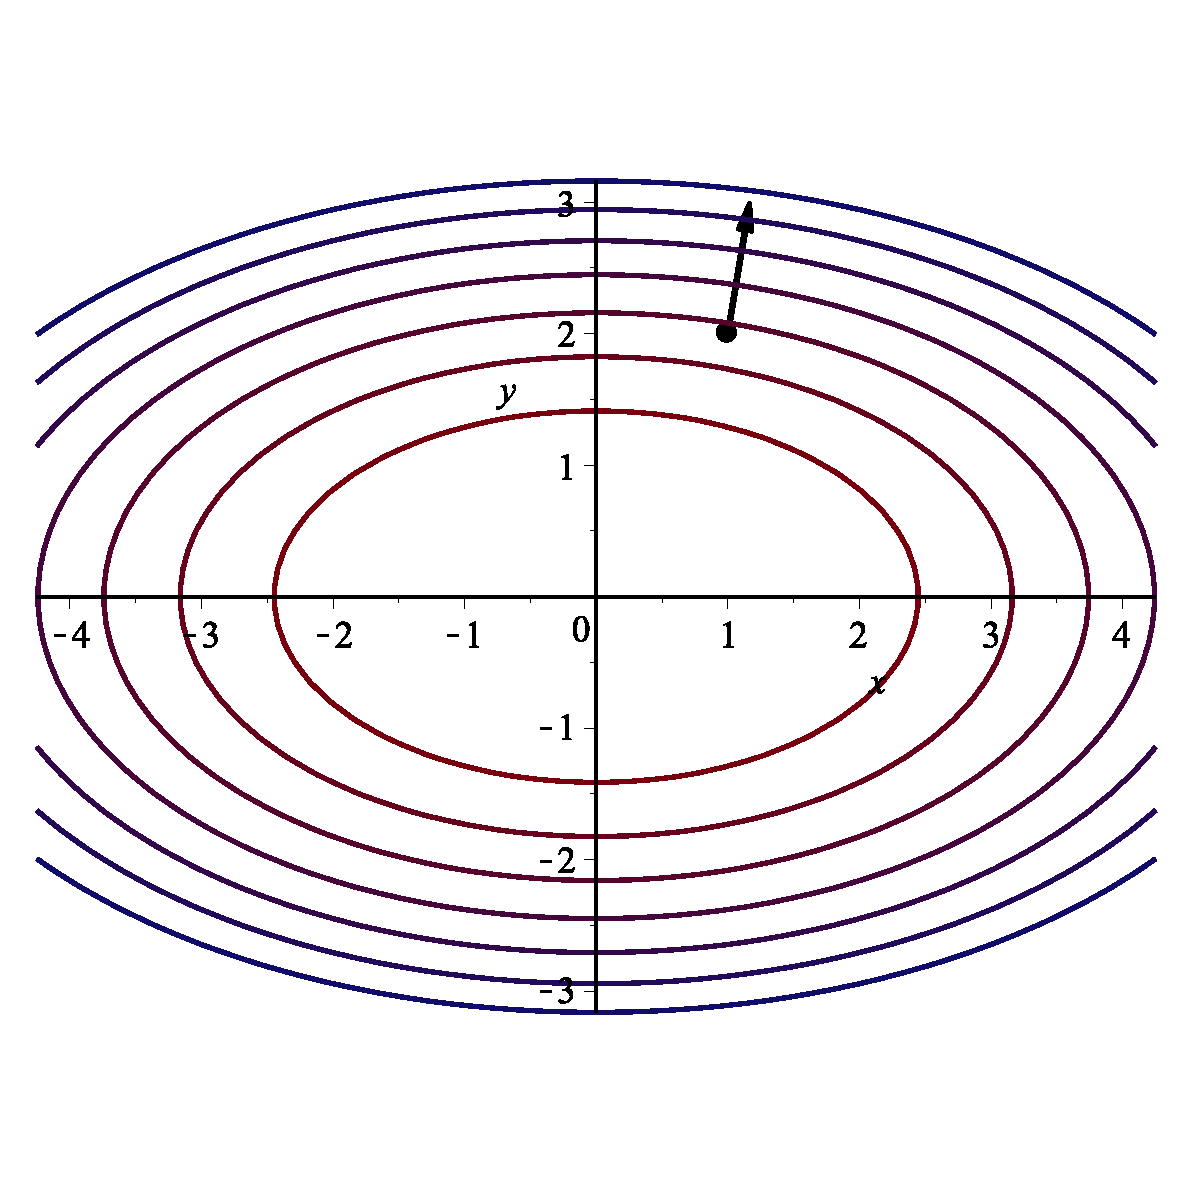
\includegraphics{10_6_6_contour_plot_gradient}}
\end{center}

\ea

\end{activitySolution}
\aftera
